\section{Hàm lượng giác}

\ % Lùi đầu dòng

\dblquote{Lượng} là đo lường, \dblquote{giác} là góc. Như vậy, \dblquote{hàm lượng giác} là hàm số đo lường góc. Trong phần này, hàm lượng giác sẽ được tiếp cận dưới góc nhìn từ đường tròn đơn vị, thay vì sử dụng tam giác vuông.

\subsection{Góc định hướng}

\ % Lùi đầu dòng

\defText{Góc không định hướng} (gọi tắt là \defText{góc}) là hình gồm hai tia có chung gốc. Gốc chung của hai tia là \defText{đỉnh} của góc. Hai tia chắn góc được gọi là \defText{cạnh} của góc.

\defText{Số đo góc} về mặt trực quan là độ mở của góc. Để đo số đo góc, chúng ta sử dụng đơn vị \defText{độ} hoặc \defText{ra-đi-an}. Gọi \defText{đường tròn đơn vị} là đường tròn có bán kính bằng $1$ đơn vị độ dài. Vẽ đường tròn đơn vị với tâm nằm ở đỉnh của góc, khi đó, số đo góc được đo bằng độ dài của cung chắn góc. Chúng ta sẽ không chứng minh tại sao mọi đường tròn lại có chu vi bằng $2\pi$ lần bán kính, nhưng sẽ sử dụng điều đó để có chu vi của đường tròn đơn vị bằng $2\pi$ đơn vị độ dài. Định nghĩa hai đơn vị đo như sau:
\begin{itemize}
   \item \defText{Độ}: Chia đường tròn làm $360$ phần bằng nhau, mỗi phần sẽ có độ dài là $\frac{2\pi}{360} = \frac{\pi}{180}$. Một cung chắn góc trên đường tròn đơn vị có đường tròn bằng này định nghĩa cho góc $1$ độ hay $\defMath{1^\circ}$.
   \item \defText{Ra-đi-an}: Một cung chắn góc trên đường tròn đơn vị có độ dài bằng $1$ định nghĩa cho góc $1$ ra-đi-an hay $\defMath{1\defText{ rad}}$.
\end{itemize}

Chúng ta tính số đo của các góc khác theo tỉ lệ với những góc đơn vị này. Như trong hình \ref{fig:toan_hoc_nen_tang:ham_luong_giac:goc_thong_dung}, góc $\textcolor{colorEmphasisCyan}{\theta_1 = \frac{\pi}{2} \text{ rad} = 90^\circ}$, góc $\textcolor{colorEmphasis}{\theta_2 = \frac{\pi}{3} \text{ rad} = 60^\circ}$ và góc $\textcolor{colorEmphasisGreen}{\theta_3 = \frac{\pi}{4} \text{ rad} = 45^\circ}$.

{
   \begin{minipage}{0.48\textwidth}
      \begin{figure}[H]
         \centering
         \begin{tikzpicture}
            \draw[color=colorEmphasisCyan, very thick] (1, 3) -- (0, 0) -- (3, 1);
            \filldraw[color=colorEmphasis] (0,0) circle (\pointSize) node[below left] {Đỉnh};
            \node[above] at (1, 3) {$y$};
            \node[above left, color=colorEmphasisCyan] at (0.5, 1.5) {Cạnh};
            \node[right] at (3, 1) {$x$};
            \node[below right, color=colorEmphasisCyan] at (1.5, 0) {Cạnh};
            \draw[color=colorEmphasisGreen] ({cos(atan(1/3))},{sin(atan(1/3))}) arc[start angle={atan(1/3)}, end angle={atan(3)}, radius=1];
            \node[above right, color=colorEmphasisGreen] at (0.65, 0.65) {$\theta$};
         \end{tikzpicture}
         \caption{Biểu diễn góc có số đo bằng $\theta$}
         \label{fig:toan_hoc_nen_tang:ham_luong_giac:sdg}
      \end{figure}
   \end{minipage}
   \hfill
   \begin{minipage}{0.48\textwidth}
      \begin{figure}[H]
         \centering
         \begin{tikzpicture}
            \draw (0, 0) -- (4, 0);
            \draw[color=colorEmphasisGreen, very thick] (0, 0) -- ({4*cos(45)}, {4*sin(45)});
            \draw[color=colorEmphasisGreen] (3, 0) arc[start angle={0}, end angle={45}, radius=3];
            \node[above right, color=colorEmphasisGreen] at ({2.9 * cos(22)}, {2.8 * sin(22)}) {$\theta_3$};
            \draw[color=colorEmphasis, very thick] (0, 0) -- ({4*cos(60)}, {4*sin(60)});
            \draw[color=colorEmphasis] (2, 0) arc[start angle={0}, end angle={60}, radius=2];
            \node[above right, color=colorEmphasis] at ({1.9 * cos(30)}, {1.8 * sin(30)}) {$\theta_2$};
            \draw[color=colorEmphasisCyan, very thick] (0, 0) -- (0, 4);
            \draw[color=colorEmphasisCyan] (1, 0) arc[start angle={0}, end angle={90}, radius=1];
            \node[right, color=colorEmphasisCyan] at ({cos(40)}, {sin(40)}) {$\theta_1$};
            \filldraw (0, 0) circle (\pointSize) node[below left] {$O$};
         \end{tikzpicture}
         \caption{Biểu diễn các góc quen thuộc}
         \label{fig:toan_hoc_nen_tang:ham_luong_giac:goc_thong_dung}
      \end{figure}
   \end{minipage}
}

Trên máy tính khoa học hiện hành còn một đơn vị nữa là \defText{gra-đi-an} được định nghĩa bằng việc chia đường tròn thành $400$ phần bằng nhau thay vì $360$ giống như độ. Khi này, chúng ta có quy đổi $$\defMath{1\defText{ grad} = 1\defText{ gon} = 1^\defText{ g} = \frac{\pi}{200}\defText{ rad}}.$$
Đơn vị này thông dụng hơn trong địa lí thay vì vật lí.
\subsection{Định nghĩa hàm số, phương trình, bất phương trình và hệ}

\ % Lùi đầu dòng

Chúng ta gọi $f$ là một \defText{hàm số} (hay \defText{hàm}) đi từ tập $X$ đến tập $Y$ khi và chỉ khi với mọi $x\in X$, gọi là \defText{tập xác định}, thông qua mối liên hệ $f$ có một và chỉ một $y\in Y$ tương ứng với $x$. Câu vừa rồi có thể được tóm gọn trong một vài kí hiệu: $$\begin{aligned}\defMath{f: X} &\defMath{\to Y} \\ \defMath{x} &\defMath{\mapsto y}\end{aligned}.$$ Khi này, chúng ta có thể viết hàm số này dưới dạng biểu thức giải tích $\defMath{y=f(x)}$, gọi $y$ là hàm của $x$. Ngoài ra, cần phải để ý rằng, thông qua định nghĩa này, mặc dù mọi $x$ trong $X$ phải có đầu ra trong $Y$, không phải mọi $y$ trong $Y$ đều phải có đầu vào trong $X$. Nói cách khác, tập tất cả các giá trị đầu ra có thể của $y=f(x)$, gọi là \defText{tập giá trị}, là tập con của tập $Y$. Nếu $x$ nằm ngoài tập giá trị $x$ thì $f(x)$ là \defText{không xác định} và không nhận bất cứ giá trị nào.

Khi chúng ta có định nghĩa hàm số thì chúng ta cũng sẽ có những khái niệm liên quan. Khi $f$ là một hàm số, thì bất cứ giá trị $a$ thuộc tập xác định để $f(a) = 0$ đều được gọi là \defText{nghiệm} của $f$. Mở rộng ra, với $f$ và $g$ là hai hàm số, bất cứ giá trị $a$ thỏa mãn $f(a) = g(a)$ thì $a$ được gọi là nghiệm của \defText{phương trình} $f(x) = g(x)$. Hơn thế nữa, nếu thay dấu $=$ trong câu vừa trước bởi các dấu $<$, $>$, $\leq$\footnote{Còn những kí hiệu khác cho dấu nhỏ hơn hoặc bằng là $\leqq$, $\leqslant$.}, $\geq$\footnote{Còn những kí hiệu khác cho dấu lơn hơn hoặc bằng là $\geqq$, $\geqslant$.}, $\neq$ thì chúng ta có định nghĩa cho nghiệm của \defText{bất phương trình}\footnote{Ngoài những dấu biểu diễn bất phương trình được kể, còn những dấu như $\nless$ (không nhỏ hơn), $\ngtr$ (không lớn hơn), $\nleq$, $\not \leqq$ hay $\nleqslant$ (không nhỏ hơn hoặc bằng), $\ngeq$, $\not \geqq$ hay $\ngeqslant$ (không lớn hơn hoặc bằng), và những dấu bị nguyền rủa $\lessgtr$ (nhỏ hơn hoặc lớn hơn), $\lesseqgtr$ hay $\lesseqqgtr$ (nhỏ hơn, lớn hơn hoặc bằng). Bạn đọc có thể sẽ muốn thêm các dấu $\not \lessgtr$ (không nhỏ hơn hay lớn hơn) và cặp dấu $\not \lesseqgtr$, $\not \lesseqqgtr$ (không nhỏ hơn, lớn hơn hay bằng) làm dấu cho bất phương trình. Tuy nhiên, trên tập số thực, $\not \lesseqgtr$ tương đương với dấu $=$, và bất phương trình với $\not \lesseqgtr$, $\not \lesseqqgtr$ thì không bao giờ thỏa mãn. Về mặt ứng dụng, ngoài những môn nặng về nền tảng của toán như đại số cao cấp, những dấu kể trên gần như không bao giờ được sử dụng.}. Lấy ví dụ, với $f$ và $g$ là hai hàm số, giá trị $a$ để $f(a) \neq g(a)$ thì $a$ được gọi là nghiệm của bất phương trình $f(x) \neq g(x)$. Kết hợp nhiều phương trình hay bất phương trình, chúng ta có một \defText{hệ}. Ví dụ:
$$
\begin{cases}
   f(x) = g(x) \\
   \alpha(y) \neq \beta(z)
\end{cases}.
$$
Để thỏa mãn hệ thì mỗi thành phần trong hệ đều phải thỏa mãn. Một khái niệm liên quan mật thiết là \defText{giải phương trình, bất phương trình, hay hệ} (để ngắn gọn, chúng ta sẽ gọi phương trình, bất phương trình và hệ thành một cụm từ chung là \dblquote{phương bất hệ}). Để làm được việc này, yêu cầu cần tìm tất cả các bộ số đẻ phương bất hệ được cho thỏa mãn. Trong trường hợp phương trình luôn đúng với mọi giá trị trong tập xác định, thì phương trình này được gọi là \defText{đẳng thức}. Một cách tương đương, nếu như bất phương trình đúng với tất cả các giá trị có thể của đầu vào thì được gọi là \defText{bất đẳng thức}.

Nếu chỉ có số với chữ không thì hàm số sẽ trở nên rất nhàm chán, cho nên người ta đã nghĩ ra phương pháp biểu diễn hàm số qua đồ thị. Để biểu diễn một hàm số $y=f(x)$ với $x$ và $y$ là hai số thực, cần vẽ tất cả các cặp tọa độ $(x; y)$ thỏa mãn hàm $f$ trên đồ thị. Trong trường hợp hàm có vô số điểm, chúng ta lấy một số giá trị để định hướng hình dạng của đồ thị và rồi sau đó nối các điểm lại\footnote{Mặc dù vậy, vẫn có trường hợp mà cách vẽ này hoàn toàn bất lực. Ví dụ như hàm Đi-rích-lê: $$f(x) =
\begin{cases}
   1 \text{ nếu } x\in \mathbb{Q} \\
   0 \text{ nếu } x\notin \mathbb{Q}
\end{cases}$$ với $\mathbb{Q}$ là tập số hữu tỉ. Hàm này liên tục nhảy bật từ $0$ đến $1$ và ngược lại, khiến cho việc vẽ đồ thị trở nên bất khả thi.}. Do hàm số biểu thị mối liên hệ giữa hai đại lượng, chúng ta dùng đồ thị hai chiều để biểu diễn mối liên hệ giữa chúng. Chúng ta sẽ lấy ví dụ cho hàm sau được cho trong bảng \ref{tab:ham_so_mot_bien:dinh_nghia:vddths} với tập xác định chỉ có $5$ số.

\begin{table}[H]
   \centering
   \begin{tabular}{|c|c|c|c|c|c|}
      \hline
      $x$ & $1$ & $2$ & $3$ & $4$ & $5$ \\
      \hline
      $y=f(x)$ & $1$ & $2$ & $5$ & $2$ & $3$ \\
      \hline
   \end{tabular}
   \caption{Ví dụ của $y = f(x)$}
   \label{tab:ham_so_mot_bien:dinh_nghia:vddths}
\end{table}

\noindent Chúng ta nhìn thấy rằng có $5$ bộ số $(x;y)$ là $(1;2)$, $(2;3)$, $(3;4)$, $(4;5)$, $(5;6)$ thỏa mãn hàm $f$ (theo đúng định nghĩa của hàm). Do đó, chúng ta có đồ thị như hình \ref{fig:ham_so_mot_bien:dinh_nghia:vddths}. 

\begin{figure}[H]
   \centering
   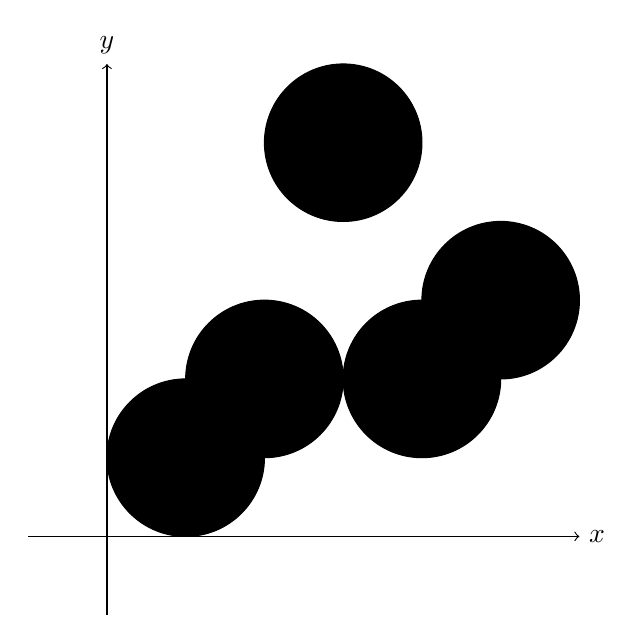
\begin{tikzpicture}
      \draw[->] (-1, 0) -- (6, 0) node[right] {$x$};
      \draw[->] (0, -1) -- (0, 6) node[above] {$y$};
      \foreach \x/\y in {1/1, 2/2, 3/5, 4/2, 5/3} {
         \filldraw (\x, \y) circle (\pointSize) node[below] {$(\x; \y)$};
      }
   \end{tikzpicture}
   \caption{Đồ thị cho ví dụ của $y = f(x)$ được cho ở bảng \ref{tab:ham_so_mot_bien:dinh_nghia:vddths}}
   \label{fig:ham_so_mot_bien:dinh_nghia:vddths}
\end{figure}

Một cách tương tự, chúng ta cũng có thể biểu diễn phương bất hệ thông qua việc vẽ đồ thị chứa các nghiệm của phương bất hệ đó. Có bao nhiêu ẩn số trong phương bất hệ, đồ thị sẽ có bấy nhiêu chiều. Giả sử như bạn đọc cần biểu diễn phương trình $x^2 - 1 = 0$ với $x$ xác định trên tập số thực. Để biểu diễn được phương trình này, trước hết cần phải thực hiện giải nó. Tác giả kì vọng bạn đọc có thể thực hiện được những biến đổi sau:
\begin{align*}
   x^2 - 1 &= 0 \\
   \iff x^2 &= 1 \\
   \iff x &\in \{-1; 1\}.
\end{align*}
Do phương trình chỉ có một ẩn nên chúng ta sẽ chọn trục số một chiều biểu diễn $x$ để thể hiện nghiệm của phương trình này, như hình \ref{fig:ham_so_mot_bien:dinh_nghia:vdgpt}.

\begin{figure}[h]
   \centering
   \begin{tikzpicture}
      \draw[->] (-3, 0) -- (3, 0) node[right] {$x$};
      \foreach \x in {-1, 1} {
         \filldraw[color=colorEmphasisCyan] (\x, 0) circle (\pointSize) node[below] {$(\x)$};
      }
   \end{tikzpicture}
   \caption{Biểu diễn nghiệm của $x^2 - 1 = 0$}
   \label{fig:ham_so_mot_bien:dinh_nghia:vdgpt}
\end{figure}

Về mặt lợi ích của việc sử dụng đồ thị, biểu diễn hình học các đại lượng đại số là một trong những cách hữu hiệu để mở rộng cảm nhận về đối tượng đang nghiên cứu.
      
\exercise Mỗi phần trong bài tập sau bao gồm mối liên hệ giữa $x$ và $y$. Trong mỗi phần, $y$ có phải là hàm của $x$ hay không? Trong trường hợp $y$ là hàm số của $x$, xác định tập xác định và tập giá trị của hàm số đó. Còn trong trường hợp ngược lại, giải thích tại sao $y$ lại không phải là hàm số của $x$.

\setcounter{subexercise}{1}
\arabic{subexercise}.
\begin{tabular}{|c|c|c|c|c|c|}
   \hline
   $x$ & $1$ & $2$ & $3$ & $4$ & $5$ \\
   \hline
   $y$ & $2$ & $3$ & $4$ & $5$ & $6$ \\
   \hline
\end{tabular};

2.
\begin{tabular}{|c|c|c|c|c|c|}
   \hline
   $x$ & $0$ & $-1$ & $1$ & $2$ & $-3$ \\
   \hline
   $y$ & $0$ & $0$ & $0$ & $0$ & $0$ \\
   \hline
\end{tabular};

3.
\begin{tabular}{|c|c|c|c|c|c|}
   \hline
   $x$ & $15$ & $15$ & $16$ & $16$ & $17$ \\
   \hline
   $y$ & $123$ & $134$ & $578$ & $426$ & $348$ \\
   \hline
\end{tabular};

4.
\begin{tabular}{|c|c|c|c|c|c|}
   \hline
   $x$ & $0$ & $-17$ & $3$ & $55$ & $-17$ \\
   \hline
   $y$ & $4586$ & $1024$ & $4586$ & $4586$ & $1024$ \\
   \hline
\end{tabular};

5. $x$ là số chỉ tháng và $y$ là số ngày trong tháng $x$.

\solution

 $y$ là hàm của $x$ với tập xác định $X = \{1; 2; 3; 4; 5\}$ và tập giá trị $Y = \{2; 3; 4; 5; 6\}$.

2. $y$ là hàm của $x$ với tập xác định $X = \{0; -1; 1; 2; -3\}$ và tập giá trị $Y = \{0\}$.

3. $y$ không phải là hàm của $x$ do khi $x$ có giá trị $15$ thì $y$ có hai giá trị $123$ và $134$.

4. $y$ là hàm của $x$ với tập xác định $X = \{0; -17; 3; 55\}$ và tập giá trị $Y = \{4586; 1024\}$. Lưu ý rằng bảng có cột bị lặp.

5. $y$ không là hàm của $x$ do khi $x = 2$ thì $y$ có hai giá trị $28$ và $29$. Mặc dù cách viết có thể ám chỉ $y=f(x)$ với $f$ là hàm số đại diện cho số ngày trong tháng, nhưng $f$ không phải là hàm số do điều ngoại lệ.

\exercise[ex:ham_so_mot_bien:dinh_nghia:intropt] Vẽ đồ thị của phương trình $\mathcal{P}$, với các định nghĩa được cho. Hàm có tập xác định là bộ số đầu vào cho ở trong bảng. Để ý số ẩn của phương trình để chọn số chiều của đồ thị cho phù hợp.

\begin{enumerate}
   \item
   \begin{tabular}{|c|c|c|c|c|c|c|}
      \hline
      $x$ & $-1$ & $1$ & $-2$ & $2$ & $-3$ & $3$\\
      \hline
      $f(x)$ & $0$ & $0$ & $4$ & $3$ & $7$ & $0$\\
      \hline
   \end{tabular} và $\mathcal{P}: f(x) = 0$;

   \item
   \begin{tabular}{|c|c|c|c|c|c|c|}
      \hline
      $x$ & $-1$ & $1$ & $-2$ & $2$ & $-3$ & $3$\\
      \hline
      $f(x)$ & $0$ & $0$ & $4$ & $3$ & $7$ & $0$\\
      \hline
   \end{tabular} và $\mathcal{P}: f(x) = x^2 - 1$;

   \item
   \begin{tabular}{|c|c|c|c|c|c|c|}
      \hline
      $x$ & $1$ & $2$ & $3$ & $4$ & $5$ & $6$\\
      \hline
      $f(x)$ & $2$ & $3$ & $5$ & $7$ & $11$ & $13$\\
      \hline
      $g(x)$ & $1$ & $3$ & $5$ & $7$ & $9$ & $11$\\
      \hline
   \end{tabular} và $\mathcal{P}: f(x) = g(x)$;

   \item
   \begin{tabular}{|c|c|c|c|c|c|c|}
      \hline
      $x$ & $1$ & $2$ & $3$ & $4$ & $5$ & $6$\\
      \hline
      $f(x)$ & $2$ & $3$ & $5$ & $7$ & $11$ & $13$\\
      \hline
      $g(x)$ & $1$ & $3$ & $5$ & $7$ & $9$ & $11$\\
      \hline
   \end{tabular} và $\mathcal{P}: f(x) = g(y)$;

   \item
   \begin{tabular}{|c|c|c|c|c|c|c|}
      \hline
      $x$ & $1$ & $2$ & $3$ & $4$ & $5$ & $6$\\
      \hline
      $f(x)$ & $2$ & $3$ & $5$ & $7$ & $11$ & $13$\\
      \hline
   \end{tabular} và $\mathcal{P}: f(x) = 2b-1$ với $b \in \mathbb{R}$;

   \item
   \begin{tabular}{|c|c|c|c|c|c|c|}
      \hline
      $x$ & $-1$ & $1$ & $-2$ & $2$ & $-3$ & $3$\\
      \hline
      $f(x)$ & $0$ & $0$ & $4$ & $3$ & $7$ & $0$\\
      \hline
   \end{tabular} và $\mathcal{P}: f(x) = f(2b - 1)$;

   \item 
   \begin{tabular}{|c|c|c|c|c|c|c|}
      \hline
      $x$ & $-1$ & $1$ & $-2$ & $2$ & $-3$ & $3$\\
      \hline
      $f(x)$ & $0$ & $0$ & $4$ & $3$ & $7$ & $0$\\
      \hline
   \end{tabular} và $\mathcal{P}: f(a) + f(b) = f(c)$;
\end{enumerate}

\solution[ex:ham_so_mot_bien:dinh_nghia:intropt]

{
   \begin{minipageindent}{0.48\textwidth}
      \indent  $\mathcal{P}$ là phương trình chỉ có một ẩn $x$, do đó đồ thị của $\mathcal{P}$ chỉ là đồ thị một chiều trên một trục số biểu diễn cho $x$.

      Có ba giá trị để $f(x)$ bằng $0$: $x\in \{-1; 1; -3\}$. Chúng ta có đồ thị của $\mathcal{P}$ ở hình \ref{fig:ham_so_mot_bien:dinh_nghia:dtp1}.
   \end{minipageindent}
   \hfill
   \begin{minipageindent}{0.48\textwidth}
      \begin{figure}[H]
         \centering
         \begin{tikzpicture}
            \draw[->] (-2, 0) -- (4, 0) node[right] {$x$};
            \foreach \x in {1, -1, 3} {
               \filldraw[color=colorEmphasisCyan] (\x, 0) circle (\pointSize) node[below] {$(\x)$};
            }
         \end{tikzpicture}
         \caption{Đồ thị phần 1 bài \ref{ex:ham_so_mot_bien:dinh_nghia:intropt}}
         \label{fig:ham_so_mot_bien:dinh_nghia:dtp1}
      \end{figure}
   \end{minipageindent}
}


{
   \begin{minipageindent}{0.48\textwidth}
      2. Tập xác định của $f(x)$ là $\{-1; 1; -2; 2; -3; 3\}$, do đó, để $\mathcal{P}$ thỏa mãn thì $x$ chỉ có thể nhận các giá trị trong vùng tập xác định.

      Kẻ bảng so sánh:
      \begin{table}[H]
         \centering
         \begin{tabular}{|c|c|c|c|c|c|c|}
            \hline
            $x$ & $-1$ & $1$ & $-2$ & $2$ & $-3$ & $3$\\
            \hline
            $f(x)$ & $0$ & $0$ & $4$ & $3$ & $7$ & $0$\\
            \hline
            $x^2-1$ & $0$ & $0$ & $3$ & $3$ & $7$ & $7$\\
            \hline
         \end{tabular}
         \caption{Giá trị của $f(x)$ và $x^2-1$ ứng với $x$}
         \label{tab:ham_so_mot_bien:dinh_nghia:values3}
      \end{table}

      Nhận thấy rằng $\mathcal{P}$ chỉ đúng khi $x\in \{-1; 1; -3; 2\}$ và chúng ta có đồ thị là hình \ref{fig:ham_so_mot_bien:dinh_nghia:dtp2}.
   \end{minipageindent}
   \hfill
   \begin{minipageindent}{0.48\textwidth}
      \begin{figure}[H]
         \centering
         \begin{tikzpicture}
            \draw[->] (-3.5, 0) -- (2.5, 0) node[right] {$x$};
            \foreach \x in {1, -1, -3, 2} {
               \filldraw[color=colorEmphasisCyan] (\x, 0) circle (\pointSize) node[below] {$(\x)$};
            }
         \end{tikzpicture}
         \caption{Đồ thị phần 2 bài \ref{ex:ham_so_mot_bien:dinh_nghia:intropt}}
         \label{fig:ham_so_mot_bien:dinh_nghia:dtp2}
      \end{figure}
   \end{minipageindent}
}

{
   \begin{minipageindent}{0.48\textwidth}
      3. Nhìn vào bảng được cho, có $f(x) = g(x)$ khi và chỉ khi $x\in \{2; 3; 4\}$. Do đó, đồ thị của $\mathcal{P}$ có được như hình \ref{fig:ham_so_mot_bien:dinh_nghia:dtp3}.
   \end{minipageindent}
   \hfill
   \begin{minipageindent}{0.48\textwidth}
      \begin{figure}[H]
         \centering
         \begin{tikzpicture}
            \draw[->] (0, 0) -- (5, 0) node[right] {$x$};
            \foreach \x in {2, 3, 4} {
               \filldraw[color=colorEmphasisCyan] (\x, 0) circle (\pointSize) node[below] {$(\x)$};
            }
         \end{tikzpicture}
         \caption{Đồ thị phần 3 bài \ref{ex:ham_so_mot_bien:dinh_nghia:intropt}}
         \label{fig:ham_so_mot_bien:dinh_nghia:dtp3}
      \end{figure}
   \end{minipageindent}
}

{
   \begin{minipageindent}{0.48\textwidth}
      4. $\mathcal{P}$ là phương trình có hai ẩn $x$ và $y$, do đó đồ thị của $\mathcal{P}$ là một mặt phẳng hai chiều. Coi như trục hoành biểu diễn cho $x$ và trục tung biểu diễn cho $y$. 

      Để có thể vẽ được đồ thị của $\mathcal{P}$, hiển nhiên nhìn ra được rằng cần phải có những điểm $(x;y)$ để hai giá trị $f(x)$ và $g(y)$ bằng nhau. Và để làm được điều đó, trước hết, chúng ta sẽ tìm xem giá trị bằng nhau của $f(x)$ với $g(y)$ này bằng bao nhiêu. Gọi chung giá trị bằng nhau này là $B_n$. Kẻ lại bảng so sánh thành bảng \ref{tab:ham_so_mot_bien:dinh_nghia:bn_values}, với $B_n$ là giá trị đầu ra và $x$, $y$ là giá trị lần lượt đưa vào hai hàm $f$ và $g$ để có giá trị đầu ra đó. Và từ đó, chúng ta có đồ thị của $\mathcal{P}$ là hình \ref{fig:ham_so_mot_bien:dinh_nghia:dtp4}.
   \end{minipageindent}
   \hfill
   \begin{minipageindent}{0.48\textwidth}
      \begin{table}[H]
         \centering
         \begin{tabular}{|c|c|c|c|c|}
            \hline
            $B_n$ & $3$ & $5$ & $7$ & $11$ \\
            \hline
            $x$ & $2$ & $3$ & $4$ & $5$ \\
            \hline
            $y$ & $2$ & $3$ & $4$ & $6$ \\
            \hline 
         \end{tabular}
         \caption{Giá trị của $x$ và $y$ ứng với $B_n$}
         \label{tab:ham_so_mot_bien:dinh_nghia:bn_values}
      \end{table}
   \end{minipageindent}
}

\begin{figure}[H]
   \centering
   \begin{tikzpicture}
      \draw[->] (0, 0) -- (3.5, 0) node[right] {$x$};
      \draw[->] (0, 0) -- (0, 3.5) node[above] {$y$};
      \filldraw[color=colorEmphasisCyan] (1, 1) circle (\pointSize) node[right] {$(2; 2)$};
      \filldraw[color=colorEmphasisCyan] (1.5, 1.5) circle (\pointSize) node[right] {$(3; 3)$};
      \filldraw[color=colorEmphasisCyan] (2.5, 3) circle (\pointSize) node[right] {$(5; 6)$};
      \filldraw[color=colorEmphasisCyan] (2, 2) circle (\pointSize) node[right] {$(4; 4)$};
   \end{tikzpicture}
   \caption{Đồ thị phần 4 bài \ref{ex:ham_so_mot_bien:dinh_nghia:intropt}}
   \label{fig:ham_so_mot_bien:dinh_nghia:dtp4}
\end{figure}

{
   \begin{minipageindent}{0.48\textwidth}
      5. $\mathcal{P}$ là phương trình có hai ẩn $x$ và $b$, do đó đồ thị của $\mathcal{P}$ là một mặt phẳng hai chiều. Coi như trục hoành biểu diễn cho $x$ và trục tung biểu diễn cho $b$.

      Tính giá trị của $b$ từ $f(x)$:
      \begin{align*}
         f(x) &= 2b - 1 \\
         \iff b &= \frac{f(x) + 1}{2}.
      \end{align*}
   \end{minipageindent}
   \hfill
   \begin{minipageindent}{0.48\textwidth}
      \begin{table}[H]
         \centering
         \begin{tabular}{|c|c|c|c|c|c|c|}
            \hline
            $x$ & $1$ & $2$ & $3$ & $4$ & $5$ & $6$\\
            \hline
            $f(x)$ & $2$ & $3$ & $5$ & $7$ & $11$ & $13$\\
            \hline
            $b$ & $\frac{3}{2}$ & $\frac{5}{2}$ & $3$ & $4$ & $6$ & $7$\\
            \hline
         \end{tabular}
         \caption{Giá trị của $b$ ứng với $x$}
         \label{tab:ham_so_mot_bien:dinh_nghia:b_values6}
      \end{table}
   \end{minipageindent}
}
Từ đây, chúng ta có thể thêm giá trị của $b$ vào bảng được cho thành bảng \ref{tab:ham_so_mot_bien:dinh_nghia:b_values6}. 

Qua bảng đó, vẽ được đồ thị của $\mathcal{P}$ như hình \ref{fig:ham_so_mot_bien:dinh_nghia:dtp5}.


\begin{figure}[H]
   \centering
   \begin{tikzpicture}
      \draw[->] (0, 0) -- (4, 0) node[right] {$x$};
      \draw[->] (0, 0) -- (0, 4) node[above] {$b$};
      \filldraw[color=colorEmphasisCyan] (0.5, 0.75) circle (\pointSize) node[below] {$\left(1; \frac{3}{2}\right)$};
      \filldraw[color=colorEmphasisCyan] (1, 1.25) circle (\pointSize) node[below] {$\left(2; \frac{5}{2}\right)$};
      \filldraw[color=colorEmphasisCyan] (1.5, 1.5) circle (\pointSize) node[right] {$(3; 3)$};
      \filldraw[color=colorEmphasisCyan] (2, 2) circle (\pointSize) node[right] {$(4; 4)$};
      \filldraw[color=colorEmphasisCyan] (2.5, 3) circle (\pointSize) node[right] {$(5; 6)$};
      \filldraw[color=colorEmphasisCyan] (3, 3.5) circle (\pointSize) node[right] {$(6; 7)$};
   \end{tikzpicture}
   \caption{Đồ thị phần 5 bài \ref{ex:ham_so_mot_bien:dinh_nghia:intropt}}
   \label{fig:ham_so_mot_bien:dinh_nghia:dtp5}
\end{figure}

{
   \begin{minipageindent}{0.48\textwidth}
      6. Nhìn vào bảng định nghĩa được cho, $f(x)$ có thể nhận các giá trị là $\{0; 3; 4; 7\}$.

      \textcolor{colorEmphasis}{Trường hợp một}: Khi $f(x) \neq 0$, chỉ có một giá trị đầu vào cho $f$ sao cho $f(x)$ đạt được giá trị đầu ra. Ví dụ, chỉ có đầu vào $x = 2$ mới có $f(x) = 3$. Do đó, khi $f(x) \neq 0$, $x = 2b-1$. Biến đổi đại số cơ bản để có $b = \frac{x + 1}{2}$. Lập bảng \ref{tab:ham_so_mot_bien:dinh_nghia:b_values7} để thấy được mối quan hệ giữa $x$ và $b$.

   \end{minipageindent}
   \hfill
   \begin{minipageindent}{0.48\textwidth}
      \begin{table}[H]
         \centering
         \begin{tabular}{|c|c|c|c|}
            \hline
            $x$ & $-2$ & $2$ & $-3$\\
            \hline
            $b = \frac{x+1}{2}$ & $-\frac{3}{2}$ & $2$ & $-1$\\
            \hline
         \end{tabular}
         \caption{Giá trị của cặp $(x; b)$ với $f(x) \neq 0$}
         \label{tab:ham_so_mot_bien:dinh_nghia:b_values7}
      \end{table}
   \end{minipageindent}
}

\textcolor{colorEmphasisCyan}{Trường hợp hai}: Khi $f(x) = 0$, $x$ và $2b-1$ có thể nhận bất cứ giá trị nào trong tập $\{-1; 1; -3\}$. Từ đó, có thể chọn $x \in \{-1; 1; 3\}$ và giải đại số để chọn $b \in \left\{\frac{-1+1}{2}; \frac{1+1}{2}; \frac{3+1}{2}\right\} = \{0; 1; 2\}$. Các cặp $(x; b)$ thỏa mãn là $(x; b)$ $\in$ $\{\left(-1; 0\right); \left(-1; 1\right); \left(-1; 2\right); \left(1; 0\right); \left(1; 1\right); \left(1; 2\right); \left(-3; 0\right); \left(-3; 1\right); \left(-3; 2\right)\}$.

Cuối cùng, kết hợp hai trường hợp, chúng ta có đồ thị cho $\mathcal{P}$:
\begin{figure}[H]
   \centering
   \begin{tikzpicture}
      \draw[->] (-4, 0) -- (3, 0) node[right] {$x$};
      \draw[->] (0, -2.5) -- (0, 2.5) node[above] {$b$};
      
      % Vẽ phần f(x) khác 0
      \filldraw[color=colorEmphasis] (-2, -1.5) circle (\pointSize) node[below] {$\left(-2; -\frac{3}{2}\right)$};
      \filldraw[color=colorEmphasis] (2, 2) circle (\pointSize) node[below] {$\left(2; 2\right)$};
      \filldraw[color=colorEmphasis] (-3, -1) circle (\pointSize) node[below] {$\left(-3; -1\right)$};
      
      \filldraw[color=colorEmphasisCyan] (-1, 0) circle (\pointSize) node[below] {$\left(-1; 0\right)$};
      \filldraw[color=colorEmphasisCyan] (1, 0) circle (\pointSize) node[below] {$\left(1; 0\right)$};
      \filldraw[color=colorEmphasisCyan] (-3, 0) circle (\pointSize) node[below] {$\left(-3; 0\right)$};
      
      \filldraw[color=colorEmphasisCyan] (-1, 1) circle (\pointSize) node[below] {$\left(-1; 1\right)$};
      \filldraw[color=colorEmphasisCyan] (1, 1) circle (\pointSize) node[below] {$\left(1; 1\right)$};
      \filldraw[color=colorEmphasisCyan] (-3, 1) circle (\pointSize) node[below] {$\left(-3; 1\right)$};
      
      \filldraw[color=colorEmphasisCyan] (-1, 2) circle (\pointSize) node[below] {$\left(-1; 2\right)$};
      \filldraw[color=colorEmphasisCyan] (1, 2) circle (\pointSize) node[below] {$\left(1; 2\right)$};
      \filldraw[color=colorEmphasisCyan] (-3, 2) circle (\pointSize) node[below] {$\left(-3; 2\right)$};
   \end{tikzpicture}
   \caption{Đồ thị phần 6 bài \ref{ex:ham_so_mot_bien:dinh_nghia:intropt}}
   \label{fig:ham_so_mot_bien:dinh_nghia:dtp7}
\end{figure}

7. $\mathcal{P}$ là phương trình có ba ẩn $a$, $b$ và $c$, do đó đồ thị của $\mathcal{P}$ là một không gian ba chiều với các trục hoành, trục tung và trục cao tương ứng là $a$, $b$ và $c$.

Theo $\mathcal{P}$, chúng ta cần phải chọn ba số trong tập giá trị của $f$ để hai trong ba số có tổng bằng số còn lại. Từ bảng, nhận thấy rằng, chỉ có thể có hai tổng $4 + 3 = 7$ và $0 + 0 = 0$.

Chúng ta cần tìm tất cả các bộ ba $(a, b, c)$ thỏa mãn $f(a) + f(b) = f(c)$. Xét hai trường hợp sau:

\textcolor{colorEmphasis}{Trường hợp một}: Tổng hai số khác 0. Để $f(a) + f(b) = f(c)$, chỉ có thể xảy ra khi $3 + 4 = 7$. Do đó, $(f(a); f(b); f(c))$ phải là $(3; 4; 7)$ hoặc $(4; 3; 7)$. Tra ngược lại bảng giá trị, chúng ta có hai nghiệm:
   \begin{itemize}
      \item $f(a)=3, f(b)=4 \implies a=2, b=-2$. Và
      \item $f(a)=4, f(b)=3 \implies a=-2, b=2$.
   \end{itemize}

Chỉ có $f(-3) = 7$ nên $c = -3$.

\textcolor{colorEmphasisCyan}{Trường hợp hai}: Tất cả bằng 0. Khi $f(a) = f(b) = f(c) = 0$, từ bảng định nghĩa, $f(x)=0$ khi $x \in \{-3; -1; 1\}$. Do đó, $a, b, c$ có thể nhận bất kỳ giá trị nào trong tập $\{-3; -1; 1\}$. Có tổng cộng $3^3 = 27$ bộ ba thỏa mãn trong trường hợp này.

Kết hợp hai trường hợp, đồ thị của $\mathcal{P}$ sẽ gồm 29 điểm trong không gian 3 chiều (2 điểm từ trường hợp 1 và 27 điểm từ trường hợp 2), được biểu diễn trong hình \ref{fig:ham_so_mot_bien:dinh_nghia:dtp8}.

\begin{figure}[H]
   \centering
   \tdplotsetmaincoords{80}{30}
   \begin{tikzpicture}[tdplot_main_coords]
      \draw[->] (-5, 0, 0) -- (2, 0, 0) node[right] {$a$};
      \draw[->] (0, -5, 0) -- (0, 4, 0) node[above] {$b$};
      \draw[->] (0, 0, -4) -- (0, 0, 2) node[above] {$c$};
      \filldraw[color=colorEmphasis] (2, -2, -3) circle (\pointSize) node[font=\scriptsize, anchor=north] {$\left(2; -2; -3\right)$};  
      \filldraw[color=colorEmphasis] (-2, 2, -3) circle (\pointSize) node[font=\scriptsize, anchor=south] {$\left(-2; 2; -3\right)$};  
      \foreach \x/\y/\z in {
         -3/-3/-3, -3/-3/-1, -3/-3/1, 
         -3/-1/-3, -3/-1/-1, -3/-1/1, -3/1/-3, -3/1/-1, -3/1/1,
         -1/-3/-3, -1/-3/-1, -1/-3/1, -1/-1/-3, -1/-1/-1, -1/-1/1,
         -1/1/-3, -1/1/-1, -1/1/1, 1/-3/-3, 1/-3/-1, 1/-3/1,
         1/-1/-3, 1/-1/-1, 1/-1/1, 1/1/-3, 1/1/-1, 1/1/1
      } {
         \filldraw[color=colorEmphasisCyan] (\x, \y, \z) circle (\pointSize);
         \node[font=\scriptsize, anchor=east, color=colorEmphasisCyan] at (\x, \y, \z) {$\left(\x; \y; \z\right)$};
      }
   \end{tikzpicture}
   \caption{Đồ thị phần 7 bài \ref{ex:ham_so_mot_bien:dinh_nghia:intropt}}
   \label{fig:ham_so_mot_bien:dinh_nghia:dtp8}
\end{figure}

\exercise[ex:ham_so_mot_bien:dinh_nghia:bpt1] Vẽ đồ thị của bất phương trình $\mathcal{P}$, với các định nghĩa đã cho. Hàm có tập xác định là bộ số đầu vào cho ở trong bảng.
\begin{enumerate}
   \item 
   \begin{tabular}{|c|c|c|c|c|c|c|}
      \hline
      $x$ & $0$ & $1$ & $2$ & $3$ & $4$ & $5$ \\
      \hline
      $f(x)$ & $-1$ & $-3$ & $-4$ & $-2$ & $-1$ & $-3$\\
      \hline
   \end{tabular} và $\mathcal{P}:f(x) \neq -3$;

   \item 
   \begin{tabular}{|c|c|c|c|c|c|c|}
      \hline
      $x$ & $-10$ & $-8$ & $-2$ & $2$ & $8$ & $10$ \\
      \hline
      $\alpha(x)$ & $4$ & $8$ & $0$ & $1$ & $6$ & $8$\\
      \hline
   \end{tabular} và $\mathcal{P}:\alpha(x) < 0$;

   \item 
   \begin{tabular}{|c|c|c|c|c|c|c|}
      \hline
      $x$ & $0$ & $6$ & $2$ & $-7$ & $-6$ & $3$ \\
      \hline
      $\beta(x)$ & $4$ & $7$ & $10$ & $3$ & $10$ & $9$\\
      \hline
   \end{tabular} và $\mathcal{P}:\beta(x) > x$;

   \item 
   \begin{tabular}{|c|c|c|c|c|c|c|}
      \hline
      $x$ & $-10$ & $-8$ & $-2$ & $2$ & $8$ & $10$ \\
      \hline
      $\alpha(x)$ & $4$ & $8$ & $0$ & $1$ & $6$ & $8$\\
      \hline
   \end{tabular},
   \begin{tabular}{|c|c|c|c|c|c|c|}
      \hline
      $x$ & $0$ & $6$ & $2$ & $-7$ & $-6$ & $3$ \\
      \hline
      $\beta(x)$ & $4$ & $7$ & $10$ & $3$ & $10$ & $9$\\
      \hline
   \end{tabular}, và $\mathcal{P}:\alpha(x) \geq 2\beta(y)$.
\end{enumerate}

\solution[ex:ham_so_mot_bien:dinh_nghia:bpt1]

{
   \begin{minipageindent}{0.48\textwidth}
      \setcounter{subexercise}{1}
      \arabic{subexercise}. Phần này tương đối đơn giản. Kiểm tra trên bảng, chúng ta thấy $f(x) = -3$ khi $x \in \{2; 5\}$. Thêm vào đó, tập xác định của $f$ là $\{0; 1; 2; 3; 4; 5\}$. Do đó, $f(x) \neq -3$ khi $x \in \{0; 1; 3; 4\}$. 

      Đồ thị của $\mathcal{P}$ là hình \ref{fig:ham_so_mot_bien:dinh_nghia:bpt1} ở bên.
   \end{minipageindent}
   \begin{minipageindent}{0.48\textwidth}
      \begin{figure}[H]
         \centering
         \begin{tikzpicture}
            \draw[->] (-1, 0) -- (5, 0) node[right] {$x$};
            \foreach \x in {0, 1, 3, 4} {
               \filldraw[color=colorEmphasisCyan] (\x, 0) circle (\pointSize) node[below] {$\left(\x\right)$};
            }
         \end{tikzpicture}
         \caption{Đồ thị phần 1 bài \ref{ex:ham_so_mot_bien:dinh_nghia:bpt1}}
         \label{fig:ham_so_mot_bien:dinh_nghia:bpt1}
      \end{figure}
   \end{minipageindent}
}

{
   \begin{minipageindent}{0.48\textwidth}
      2. Tra bảng trực tiếp, các giá trị $\alpha(x)$ không bao giờ nhỏ hơn $0$. Chúng ta không xét giá trị $x$ ngoài bảng do không thuộc tập xác định của hàm $\alpha$. Do đó, $\alpha(x) < 0$ là bất phương trình vô nghiệm.

      Và qua đó, vẽ được đồ thị của $\mathcal{P}$ là trục không đánh dấu như hình \ref{fig:ham_so_mot_bien:dinh_nghia:bpt2}.
   \end{minipageindent}
   \begin{minipageindent}{0.48\textwidth}
      \begin{figure}[H]
         \centering
         \begin{tikzpicture}
            \draw[->] (-1, 0) -- (5, 0) node[right] {$x$};
         \end{tikzpicture}
         \caption{Đồ thị phần 2 bài \ref{ex:ham_so_mot_bien:dinh_nghia:bpt1}}
         \label{fig:ham_so_mot_bien:dinh_nghia:bpt2}
      \end{figure}
   \end{minipageindent}
}

3. Xét trên tập xác định của $\beta$, chúng ta có $\beta(x) > x$ với mọi $x$ nằm trên bảng được cho. Một cách đơn giản, chúng ta có đồ thị là hình \ref{fig:ham_so_mot_bien:dinh_nghia:bpt3}.

\begin{figure}[H]
   \centering
   \begin{tikzpicture}
      \draw[->] (-8, 0) -- (8, 0) node[right] {$x$};
      \foreach \x in {0, 6, 2, -7, -6, 3} {
         \filldraw[color=colorEmphasisCyan] (\x, 0) circle (\pointSize) node[below] {$\left(\x\right)$};
      }
   \end{tikzpicture}
   \caption{Đồ thị phần 3 bài \ref{ex:ham_so_mot_bien:dinh_nghia:bpt1}}
   \label{fig:ham_so_mot_bien:dinh_nghia:bpt3}
\end{figure}

4. Chúng ta có thể kiểm tra trực tiếp $36$ cặp $(x; y)$ và sau đó vẽ đồ thị. Sau đây, tác giả sẽ chỉ những góc nhìn để có thể giảm số trường hợp cần kiểm tra.

Để ý rằng, giá trị lớn nhất có thể của $\alpha(x)$ là $8$. Mặt khác, để $\mathcal{P}$ thỏa mãn thì
\begin{align*}
   \alpha(x) &\geq 2\beta(y) \\
   \iff \beta(y) &\leq \frac{\alpha(x)}{2}. \\
\end{align*}
Qua đó, giá trị lớn nhất có thể của $\beta(y)$ là $4$. Theo bảng định nghĩa, $\beta(y)$ chỉ có thể nhận hai giá trị là $3$ hoặc $4$. 

\textcolor{colorEmphasisCyan}{Trường hợp một}: $\beta(y) = 3 \iff y = -7$. Khi này, để $\alpha(x) \geq 2\beta(x)$ hay $\alpha(x) \geq 6$ thì $\alpha(x)$ có thể nhận giá trị $8$ hoặc $6$. Do đó,
\begin{align*}
   &\alpha(x) = 6 \implies x = 8;\\
   &\alpha(x) = 8 \implies x \in \{-8; 10\}.
\end{align*}

\textcolor{colorEmphasis}{Trường hợp hai}: $\beta(y) = 4 \iff y = 0$. Khi này, để $\alpha(x) \geq 8$ thì $\alpha(x)$ chỉ có thể nhận bằng $8$. Do đó, $x \in \{-8; 10\}$.

Từ đây, chúng ta có đồ thị \ref{fig:ham_so_mot_bien:dinh_nghia:bpt4}.

\begin{figure}[H]
   \centering
   \begin{tikzpicture}
      \draw[->] (-4, 0) -- (4, 0) node[right] {$x$};
      \draw[->] (0, -3) -- (0, 0) node[above] {$y$};
      \foreach \x/\y/\pos in {8/-7/above, -8/-7/below, 10/-7/below} {
         \filldraw[color=colorEmphasisCyan] (\x/3, \y/3) circle (\pointSize) node [\pos] {$\left(\x; \y\right)$};
      }
      \foreach \x/\y/\pos in {-8/0/below, 10/0/below} {
         \filldraw[color=colorEmphasis] (\x/3, \y/3) circle (\pointSize) node [\pos] {$\left(\x; \y\right)$};
      }
   \end{tikzpicture}
   \caption{Đồ thị phần 4 bài \ref{ex:ham_so_mot_bien:dinh_nghia:bpt1}}
   \label{fig:ham_so_mot_bien:dinh_nghia:bpt4}
\end{figure}

\exercise[ex:ham_so_mot_bien:dinh_nghia:hpt1] Vẽ đồ thị của hệ phương trình $\mathcal{P}$, với các định nghĩa đã cho. Hàm có tập xác định là bộ số đầu vào cho ở trong bảng.
\begin{enumerate}
   \item 
   \begin{tabular}{|c|c|c|c|c|c|c|}
      \hline
      $x$ & $0$ & $1$ & $2$ & $3$ & $4$ & $5$ \\
      \hline
      $f(x)$ & $-1$ & $-1$ & $-1$ & $-2$ & $-3$ & $-3$\\
      \hline
   \end{tabular},
   \begin{tabular}{|c|c|c|c|c|c|c|}
      \hline
      $y$ & $0$ & $-2$ & $4$ & $-6$ & $8$ & $-10$\\
      \hline
      $g(y)$ & $-1$ & $-2$ & $-3$ & $-7$ & $-8$ & $-9$\\
      \hline
   \end{tabular},

   \noindent\begin{tabular}{|c|c|c|c|c|c|c|}
      \hline
      $z$ & $-1$ & $1$ & $-2$ & $0$ & $-4$ & $4$\\
      \hline
      $h(z)$ & $2$ & $1$ & $0$ & $-1$ & $-2$ & $-3$\\
      \hline
   \end{tabular} và $\mathcal{P}:f(x) = g(x) = h(x)$;

   \item
   \begin{tabular}{|c|c|c|c|c|c|c|}
      \hline
      $x$ & $0$ & $1$ & $2$ & $3$ & $4$ & $5$ \\
      \hline
      $f(x)$ & $-1$ & $-1$ & $-1$ & $-2$ & $-3$ & $-3$\\
      \hline
   \end{tabular},
   \begin{tabular}{|c|c|c|c|c|c|c|}
      \hline
      $y$ & $0$ & $-2$ & $4$ & $-6$ & $8$ & $-10$\\
      \hline
      $g(y)$ & $-1$ & $-2$ & $-3$ & $-7$ & $-8$ & $-9$\\
      \hline
   \end{tabular},

   \noindent\begin{tabular}{|c|c|c|c|c|c|c|}
      \hline
      $z$ & $-1$ & $1$ & $-2$ & $0$ & $-4$ & $4$\\
      \hline
      $h(z)$ & $2$ & $1$ & $0$ & $-1$ & $-2$ & $-3$\\
      \hline
   \end{tabular} và $\mathcal{P}:f(a) = g(b) = h(c)$;

   \item
   \begin{tabular}{|c|c|c|c|c|c|c|}
      \hline
      $x$ & $0$ & $1$ & $2$ & $3$ & $4$ & $5$ \\
      \hline
      $f(x)$ & $-1$ & $-1$ & $-1$ & $-2$ & $-3$ & $-3$\\
      \hline
   \end{tabular},
   \begin{tabular}{|c|c|c|c|c|c|c|}
      \hline
      $y$ & $0$ & $-2$ & $4$ & $-6$ & $8$ & $-10$\\
      \hline
      $g(y)$ & $-1$ & $-2$ & $-3$ & $-7$ & $-8$ & $-9$\\
      \hline
   \end{tabular},

   \noindent\begin{tabular}{|c|c|c|c|c|c|c|}
      \hline
      $z$ & $-1$ & $1$ & $-2$ & $0$ & $-4$ & $4$\\
      \hline
      $h(z)$ & $2$ & $1$ & $0$ & $-1$ & $-2$ & $-3$\\
      \hline
   \end{tabular} và $\mathcal{P}:\begin{cases}f(o) = g(p)\\f(p + 1) = h(q)\end{cases}$.

   \item
   \begin{tabular}{|c|c|c|c|c|c|c|}
      \hline
      $x$ & $0$ & $1$ & $2$ & $3$ & $4$ & $5$ \\
      \hline
      $f(x)$ & $-1$ & $-1$ & $-1$ & $-2$ & $-3$ & $-3$\\
      \hline
   \end{tabular},
   \begin{tabular}{|c|c|c|c|c|c|c|}
      \hline
      $y$ & $0$ & $-2$ & $4$ & $-6$ & $8$ & $-10$\\
      \hline
      $g(y)$ & $-1$ & $-2$ & $-3$ & $-7$ & $-8$ & $-9$\\
      \hline
   \end{tabular},

   \noindent\begin{tabular}{|c|c|c|c|c|c|c|}
      \hline
      $z$ & $-1$ & $1$ & $-2$ & $0$ & $-4$ & $4$\\
      \hline
      $h(z)$ & $2$ & $1$ & $0$ & $-1$ & $-2$ & $-3$\\
      \hline
   \end{tabular} và $\mathcal{P}:\begin{cases}f(m) = n\\g(n) = h(w)\end{cases}$.
\end{enumerate}

\solution[ex:ham_so_mot_bien:dinh_nghia:hpt1]

\setcounter{subexercise}{1}
\arabic{subexercise}. Giá trị đầu vào để $f, g, h$ đều có cùng một đầu ra là $x\in\{0;4\}$. Vậy, chúng ta có đồ thị như hình \ref{fig:hpt11}.

\begin{figure}[H]
   \centering
   \begin{tikzpicture}
      \draw[->] (-1, 0) -- (5, 0) node[right] {$x$};
      \filldraw[color=colorEmphasisCyan] (0, 0) circle (\pointSize) node[below] {$(0)$};
      \filldraw[color=colorEmphasisCyan] (4, 0) circle (\pointSize) node[below] {$(4)$};
   \end{tikzpicture}
   \caption{Đồ thị phần 1 bài \ref{ex:ham_so_mot_bien:dinh_nghia:hpt1}}
   \label{fig:hpt11}
\end{figure}

2. Trước hết, cần tìm những giá trị chung trong tập giá trị của $f, g, h$. Nhận thấy rằng, có $-1, -2$ và $-3$ là những giá trị chung trong đó. 
\begin{itemize}
   \item Với đầu ra là $-1$, chúng ta có $f(a) = g(b) = h(c) = -1$. Từ đó, chúng ta có $a \in \{0; 1; 2\}$ và $b = c = 0$.
   \item Trong trường hợp kết quả của hàm là $-2$, $f(a) = g(b) = h(c) = -2$. Từ đó, bộ ba $\left(a; b; c\right)$ có giá trị là $(3; -2; -4)$.
   \item Trong trường hợp kết quả của hàm là $-3$, $f(a) = g(b) = h(c) = -3$. Từ đó, $\left(a; b; c\right)$ $\in \left\{\left(4; 4; 4\right); \left(5; 4; 4\right)\right\}$.
\end{itemize}
Kết hợp ba trường hợp, xây dựng không gian tọa độ, chúng ta có hình \ref{fig:hpt12}.

\begin{figure}[H]
   \centering
   \tdplotsetmaincoords{80}{-10}
   \begin{tikzpicture}[tdplot_main_coords]
      \draw[->] (-1.5, 0, 0) -- (3, 0, 0) node[right] {$a$};
      \draw[->] (0, -1, 0) -- (0, 2.5, 0) node[above] {$b$};
      \draw[->] (0, 0, -2.5) -- (0, 0, 2.5) node[above] {$c$};
      \foreach \x/\y/\z/\pos in {
         0/0/0/below left,
         1/0/0/above,
         2/0/0/below} {
            \filldraw[color=colorEmphasisCyan] ({\x/2}, {\y/2}, {\z/2}) circle (\pointSize) node[\pos] {$\left(\x; \y; \z\right)$};
      }
      \filldraw[color=colorEmphasis] (1.5, -1, -2) circle (\pointSize) node[above] {$\left(3; -2; -4\right)$};
      \foreach \x/\y/\z/\pos in {
         4/4/4/above,
         5/4/4/below} {
            \filldraw[color=colorEmphasisGreen] ({\x/2}, {\y/2}, {\z/2}) circle (\pointSize) node[\pos] {$\left(\x; \y; \z\right)$};
      };
   \end{tikzpicture}
   \caption{Đồ thị phần 2 bài \ref{ex:ham_so_mot_bien:dinh_nghia:hpt1}}
   \label{fig:hpt12}
\end{figure}

3. Để $f$ và $g$ nhận cùng một giá trị thì giá trị đầu ra đó, theo bảng định nghĩa được cho, kết quả mà hàm trả ra phải là $-1$, $-2$ hoặc $-3$.
\begin{itemize}
   \item Tại $f(o) = g(p) = -1$, $o \in \{0; 1; 2\}$ và $p = 0$. Từ đó, $f(p + 1) = f(1) = -1$. Khi này, $h(q) = -1 \iff q = 0$.
   \item Tại $f(o) = g(p) = -2$, sau khi tra bảng, chúng ta thấy được rằng $\begin{cases}o = 3\\p = -2\end{cases}$; suy ra $f(p + 1) = f(-1)$, Tuy nhiên, $-1$ không thuộc tập xác định của $f$. Vậy, chúng ta sẽ loại trường hợp này.
   \item Tại $f(o) = g(p) = -3$, $o \in \{4; 5\}$ và $p = 4$. Từ đó, $f(p + 1) = f(5) = -3$. Khi này, $h(q) = -3 \iff q = 4$.
\end{itemize}
Cuối cùng, vẽ đồ thị để được hình \ref{fig:hpt13}.

\begin{figure}[H]
   \tdplotsetmaincoords{80}{-10}
   \centering
   \fbox{
      \begin{tikzpicture}[tdplot_main_coords]
         \draw[->] (-1, 0, 0) -- (3, 0, 0) node[right] {$o$};
         \draw[->] (0, -1, 0) -- (0, 2.5, 0) node[above] {$p$};
         \draw[->] (0, 0, -1) -- (0, 0, 2.5) node[above] {$q$};
         \foreach \x/\y/\z/\pos in {
            0/0/0/below left,
            1/0/0/above,
            2/0/0/below} {
               \filldraw[color=colorEmphasisCyan] ({\x/2}, {\y/2}, {\z/2}) circle (\pointSize) node[\pos] {$\left(\x; \y; \z\right)$};
         }
         \foreach \x/\y/\z/\pos in {
            4/4/4/above,
            5/4/4/below} {
               \filldraw[color=colorEmphasisGreen] ({\x/2}, {\y/2}, {\z/2}) circle (\pointSize) node[\pos] {$\left(\x; \y; \z\right)$};
         };
      \end{tikzpicture}
   }
   \caption{Đồ thị phần 3 bài \ref{ex:ham_so_mot_bien:dinh_nghia:hpt1}}
   \label{fig:hpt13}
\end{figure}

4. Theo đề, chúng ta cần tìm những bộ $(m;n;w)$ thỏa mãn $\mathcal{P}$, trong đó có $g(n) = h(w)$. Cho nên, $n$ phải thuộc tập xác định của $g$. Nhìn vào bảng, tập xác định đó là $\{0; -2; 4; -6; 8; -10\}$. Tuy nhiên, cũng có $f(m) = n$, cho nên $n$ vừa phải thuộc tập giá trị của $f$, hay $n \in \{-1; -2; -3\}$. Lấy giao của hai tập đó, chúng ta có $n = -2$. Từ đó, giải $f(m) = -2$ để có $m = 3$. Thêm vào đó, $h(w) = g(-2) = -2 \iff w = -4$.

Bộ số duy nhất thỏa mãn hệ phương trình $\mathcal{P}$ là $\left(m; n; w\right) = \left(3; -2; -4\right)$. Đồ thị của $\mathcal{P}$ là hình \ref{fig:hpt14}.

\begin{figure}[H]
   \tdplotsetmaincoords{80}{20}
   \centering
   \fbox{
      \begin{tikzpicture}[tdplot_main_coords]
         \draw[->] (-0.5, 0, 0) -- (2, 0, 0) node[right] {$m$};
         \draw[->] (0, -1.5, 0) -- (0, 0.5, 0) node[above] {$n$};
         \draw[->] (0, 0, -2.5) -- (0, 0, 0.5) node[above] {$w$};
         \filldraw[color=colorEmphasisCyan] (1.5, -1, -2) circle (\pointSize ) node[above] {$\left(3; -2; -4\right)$};
      \end{tikzpicture}
   }
   \caption{Đồ thị phần 4 bài \ref{ex:ham_so_mot_bien:dinh_nghia:hpt1}}
   \label{fig:hpt14}
\end{figure}
\subsection{Hàm lượng giác trong tam giác vuông}

\ % Lùi đầu dòng

{
   \begin{minipageindent}{0.48\textwidth}
      \begin{figure}[H]
         \centering
         \begin{tikzpicture}
            \pgfmathsetmacro{\xC}{2}
            \pgfmathsetmacro{\yC}{4}
            \pgfmathsetmacro{\xB}{0}
            \pgfmathsetmacro{\yB}{0}
            \pgfmathsetmacro{\slope}{(\xC - \xB)/(\yB - \yC)}
            \pgfmathsetmacro{\leftShift}{\guideLineLength*1 / sqrt((\slope)^2+1)}
            \pgfmathsetmacro{\upShift}{\guideLineLength*(\slope) / sqrt((\slope)^2+1)}

            \draw[\guideLineThickness] (\xC, \yC) -- ({\xC - \leftShift}, {\yC - \upShift});
            \draw[\guideLineThickness] (\xB, \yB) -- ({\xB - \leftShift}, {\yB - \upShift});
            \draw[measuring arrow, color=colorEmphasisCyan] ({\xC - \leftShift / 2}, {\yC - \upShift / 2}) -- ({\xB - \leftShift / 2}, {\yB - \upShift / 2}) node[midway, above left] {$h$};
            
            \draw[very thick, color=colorEmphasisCyan] (\xB, \yB) -- (\xC, \yC);

            \draw[very thick, color=colorEmphasis] (0,0) -- (2,0);
            \draw[\guideLineThickness] (0,0) -- (0, -\guideLineLength);
            \draw[\guideLineThickness] (2,0) -- (2, -\guideLineLength);
            \draw[measuring arrow, color=colorEmphasis] (0, -\guideLineLength / 2) -- (2, -\guideLineLength / 2) node[midway, below] {$k$};

            \draw[very thick, color=colorEmphasisGreen] (2,0) -- (2,4);
            \draw[\guideLineThickness] (2,0) -- (2+\guideLineLength, 0);
            \draw[\guideLineThickness] (2,4) -- (2+\guideLineLength, 4);
            \draw[measuring arrow, color=colorEmphasisGreen] (2+\guideLineLength / 2, 0) -- (2+\guideLineLength / 2, 4) node[midway, right] {$d$};

            \filldraw (0,0) circle (\pointSize) node[below left] {$B$};
            \filldraw (2,0) circle (\pointSize) node[below right] {$A$};
            \filldraw (2,4) circle (\pointSize) node[above] {$C$};
         \end{tikzpicture}
      \end{figure}
   \end{minipageindent}
   \hfill
   \begin{minipageindent}{0.48\textwidth}
      Trong trường hợp góc $\theta$ thỏa mãn $0 < \theta < 90^\circ$, tồn tại $\triangle ABC$ vuông tại $A$ với $\angle BAC = \theta$.  
   \end{minipageindent}
}

\subsection{Tính chất hàm lượng giác}

\ % Lùi đầu dòng

Sử dụng hình \ref{fig:toan_hoc_nen_tang:dinh_nghia:dn_sin_cos}, bởi vì $\triangle OCP$ vuông tại $C$ có $OP$ là cạnh huyền nên:
\begin{align}
   &\begin{cases}
      CP \leq OP \\
      -CP \leq OP \equationexplanation{Trong trường hợp $P$ nằm ở bên trái trục tung.}
   \end{cases} \nonumber\\
   \iff &-OP \leq CP \leq OP \label{eq:toan_hoc_nen_tang:ham_luong_giac:dinh_nghia:dn_sin_cos}
\end{align}
Theo định nghĩa, $CP = \cos \left(\theta\right)$, và do $P$ nằm trên đường tròn đơn vị nên $OP = 1$. Qua đó, kết hợp với \refeq{eq:toan_hoc_nen_tang:ham_luong_giac:dinh_nghia:dn_sin_cos} để có
\begin{equation*}
   \defMath{-1 \leq \cos \left(\theta\right) \leq 1}.
\end{equation*}
Tương tự, chúng ta cũng có $\defMath{-1 \leq \sin \left(\theta\right) \leq 1}$.


